%\usepackage{graphicx}

\subsection{Prototyping (!)}
In the manufacturing cycle, prototyping plays a crucial role. It assesses the fit, functionality,
and form of the parts being prototyped. This phase is important because it provides a clear idea of 
the final product's appearance and allows for the identification of unnecessary elements in the design. 
By addressing these issues during the prototyping stage, it saves time and money that would otherwise be 
spent making corrections during the production phase.
\newline \newline
Prototyping can be traced back to 1859, when a method known as photosculpture was invented by 
the French inventor Francois Willeme \cite{Lengua2017}. By surrounding an object with twenty-four 
cameras, each separated by 15 degrees, and taking photographs simultaneously, each photograph could 
be projected onto a screen. Using the images, a pantograph, and pieces of wood, 3D sculptures could 
be recreated from the photographs. This method of 3D prototyping enjoyed brief success but was eventually 
abandoned due to its labor-intensive nature.
\newline \newline
Further on, in 1981, Hideo Kodama, who worked at the Nagoya Municipal Industrial Research 
Institute in Japan, released a paper describing what is likely the first 3D-printed object 
in history \cite{Lengua2017}. The paper outlines a system called ``Automatic Method for Fabricating 
Cubic Shapes.'' This method involved using a photo-hardening polymer to fabricate solid models by 
stacking layers 2 mm thick on top of each other, thereby creating the first 3D-printed object. 
Similarly, Charles Hull developed stereolithography in 1986 \cite{SU20181}. This method involves 
solidifying a liquid material when it is exposed to UV light, based on cross-sections of a 3D model.
Unlike Hideo Kodama, Charles Hull patented his method and achieved greater academic and commercial 
success. However, Hideo Kodama was eventually awarded the Rank Prize, a prestigious award given to 
outstanding inventors, which he shared with Hull.
\newline \newline
For prototyping, 3D printing is a widely used tool across various industries, including aviation,
medical, automotive, etc. This technology is based on the concept of solidifying materials. 
Typically, the process begins with the creation of a 3D model in CAD or a similar system. 
These programs generate a file containing instructions for a rapid prototyping machine, usually 
a 3D printer, to create the 3D model in solid form \cite{sriharsha2018rapid}. There are several 
techniques for producing a prototype in the realm of 3D printing, including:
\begin{itemize}
    \item Stereo lithography
    \item Selective Laser Sintering
    \item Fused Deposition Modeling
\end{itemize}
While these technologies differ in their specific processes, they share similar advantages, such as 
reducing product development and manufacturing costs, thereby increasing competitiveness 
\cite{PHAM19981257}. Initially, these technologies and rapid prototyping were only accessible to 
large corporate firms, but today, 3D printers have become affordable for private individuals as well. 
Before the widespread availability of 3D printing, prototyping required skilled engineers to work from 
2D drawings.


\subsection{Virtual Reality (!)}
Virual reality  is a tool that artificialy simualtes our senses. While the technology might seem new, 
the first VR technology was introdoced by Ivan sutherland in 1968 \cite{lavalle2023virtual}. Today the VR
industry is worth billions of dollars and is found in many industries
\subsection{Virtual Reality Prototyping (!)}
\subsection{3D rendering tools (!)}
3D rendering is used in multiple industries for various purposes, such as creating and animating special 
effects in movies, virtual prototyping, developing games, etc. Although the core technology behind 3D 
rendering is quite complex and requires advanced in-depth knowledge of coordinate systems, including the 
Cartesian coordinate system, and graphics along with complex algorithms, only a limited number of people 
possess this expertise. Consequently, software tools for simplifying the 3D rendering process have naturally 
emerged. Depending on the purpose, different tools have arisen: for 3D modeling, CAD has become a suitable 
option, while for 3D environments, Blender or Unreal Engine are more appropriate.
\newline \newline
These tools eliminate an element of manual editing that would have otherwise been tedious. For the purpose 
of creating a virtual prototyping environment, 3D rendering tools can be highly beneficial in that they 
save a significant amount of time in setting up the 3D VR environment
\subsection{Unreal Engine (!)}
The development of 3D environments, which are the primary type of environment for VR, can be accomplished 
using multiple tools. However, one tool that has stood out is Unreal Engine. Originally created as a game 
engine, Unreal Engine is now utilized in various industries, as mentioned earlier. There are multiple 
versions of Unreal Engine, and at the time of writing, version 5.3.2 is the latest stable release. In 
Unreal Engine 5, the actual engine and projects are organized into separate folders, with the editor 
serving as a bridge yet remaining part of the engine. A simple illustration of this organization is 
shown in Figure \ref{figure 1}.
\begin{figure}
    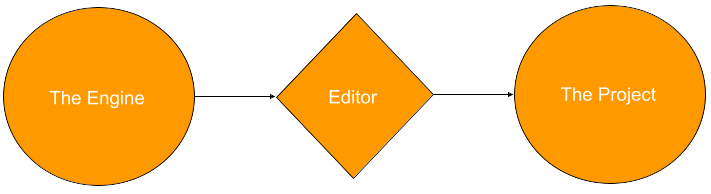
\includegraphics[width=1.0\textwidth]{SimpleEngineToProject.png}
    \centering
    \label{figure 1}
    \caption[short]{Figure 1: Engine structure}
\end{figure}
\newline \newline
With Unreal Engine, a set of default environments is available to choose from as a starting point. 
These environments are tailored to different use cases, such as film and video production, 
architecture, simulations, and so on. For virtual reality, there are default environments 
specifically designed to allow the editor to preview the environment using a VR headset.

\subsection{Unreal Engine in Automotive Industry (!)}
To justify the use of Unreal Engine in this project it is a good idea to look how Unreal Engine is used in 
other parts of the automotive industry and what advantages it brings and if it in any way brings disadvanatges
and how thoose should be taken into consideration. 
\newline \newline
One potentially obvious use case for Unreal Engine in the automotive industry is vehicle design. Traditionally, 
car companies would create a design and conduct user surveys on it. By using VR, it becomes possible to let a 
user evaluate a design while simultaneously tracking where their attention is directed. The results revealed 
that a user could respond to the survey with explanations that might not accurately reflect where their 
attention was primarily focused. For instance, one user evaluated a car model in VR and commented that 
the tires "looked sporty," yet it was found that they spent very little time actually looking at the 
wheels. Instead, other parts of the car received more attention ultimately \cite{UnrealEngine_2022}.

%Multiple car brands uses Unreal Engine for different puropses. Volvo, a var brand with emphasis on safety
%uses Unreal Engine to vizualise and enhance sensor and safety. A part from this thet also prototype human
%to machine intercation (HMI) functionality
\subsection{Einride (!)}
